% Universidade Aberta
% Template TeX para relatório de trabalhos
% 2025
%
%
% Dados para a capa
\newcommand{\Titulo}{Planeamento e Desenvolvimento de Sistemas de Informação}
\newcommand{\SubTitulo}{Trabalho Grupo - Topico 3}
\newcommand{\Ano}{2025}
\newcommand{\Autor}{
    Pedro Morais - 2401849 \\
    Hugo Gonçalves - 2100562 \\
    Pedro Moro - 2001642 \\
    Luis Peixoto - 2402741 \\
}
%
%
\documentclass[12pt,a4paper,final]{article}
\usepackage{csquotes}
\usepackage[portuguese]{babel}
\usepackage{polyglossia}
\setdefaultlanguage{portuguese}
\usepackage{graphicx}
\graphicspath{ {./images/} }
\usepackage[a4paper,top=3cm,bottom=3cm,left=3.5cm,right=2cm]{geometry}
\usepackage{booktabs}
\setmainfont{Times New Roman}
\defaultfontfeatures{Ligatures=TeX}
\usepackage[pdfauthor=\Autor,
    pdftitle=\Titulo,
    colorlinks=true,
    linkcolor=black,
    citecolor=black,
    bookmarksopen=true]{hyperref}
\hypersetup{colorlinks, citecolor=black, urlcolor=black}
\usepackage{bookmark}
\usepackage[style=apa, backend=biber, sortcites, url=true, language=portuguese]{biblatex}
\usepackage{fontspec}
\DeclareLanguageMapping{portuguese}{portuguese-apa}
\addbibresource{ref.bib}
\renewcommand{\baselinestretch}{1.5}
\begin{document}
    \title{\Titulo}
    \author{\Autor}
    \date{\Ano}
    \pagenumbering{gobble}
    \begin{titlepage}
        \begin{center}
            \vspace*{4cm}

            \textbf{\large UNIVERSIDADE ABERTA}

            \textbf{\large UNIVERSIDADE DE TRÁS-OS-MONTES E ALTO DOURO}

            \vspace{1cm}

            \begin{minipage}{0.4\textwidth}
                \centering
                
\includegraphics[width=0.8\textwidth]{uab}
            \end{minipage}
            \begin{minipage}{0.4\textwidth}
                \centering
                
\includegraphics[width=0.8\textwidth]{utad}
            \end{minipage}

            \vspace{1.5cm}

            \textbf{\large \Titulo}

            \textbf{\large \SubTitulo}

            \vspace{1.5cm}

            \textbf{\large \Autor}

            \vspace{2cm}

            \textbf{\large Mestrado em Engenharia Informática e Tecnologia Web}
            \vfill
            \textbf{\Ano}
        \end{center}
    \end{titlepage}
    \renewcommand{\contentsname}{Índice}
    \cleardoublepage
    \pagenumbering{roman}
    \tableofcontents
    \newpage
    \listoffigures
    \newpage
    \cleardoublepage
    \pagenumbering{arabic}


    \section{Introdução}\label{sec:introducao}
    O presente relatório tem como objetivo a caracterização da arquitectura empresarial da Direção Municipal de Higiene Urbana (DMHU), unidade funcional da Câmara Municipal de Lisboa (CML), no seu estado atual ("AS-IS").
    Este trabalho insere-se no âmbito da unidade curricular de Planeamento e Desenvolvimento de Sistemas de Informação (PDSI), e serve de base para uma futura transformação da organização.

    \section{Contexto Organizacional e Atores Envolvidos}\label{sec:contexto-organizacional-e-atores-envolvidos}

    A DMHU integra-se na estrutura funcional da Câmara Municipal de Lisboa, sendo responsável pela gestão de resíduos e higiene urbana.
    \begin{itemize}
        \item Cidadãos de Lisboa (reclamações, ocorrências, pedidos);
        \item Juntas de Freguesia (intervenções locais, eventos);
        \item Entidades Reguladoras (ex: ERSAR);
        \item Polícia Municipal (fiscalização);
        \item Fornecedores e prestadores de serviços.
    \end{itemize}

    \begin{figure}[h!]
        \centering
        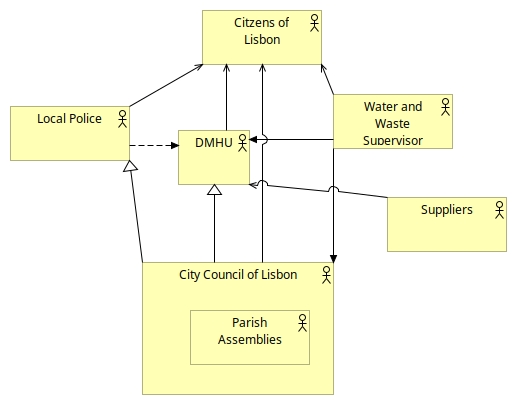
\includegraphics[width=0.25\textwidth]{Q1 - DHMU Context}
        \caption{Modelo ArchiMate — Cooperação com Atores Externos}
        \label{fig:1}
    \end{figure}

    Esta análise responde à \textbf{Questão 1 — DMHU Context (Actor Cooperation Viewpoint)}.

    \newpage

    \section{Produtos e Serviços Prestados}\label{sec:produtos-e-servicos-prestados}

    A DMHU presta os seguintes serviços à cidade:
    \begin{itemize}
        \item Higiene Urbana;
        \item Limpeza Urbana;
        \item Projetos de Higiene;
        \item Transporte;
        \item Sensibilização Ambiental;
        \item Gestão de Garagens e Oficinas.
    \end{itemize}

    \begin{figure}[h!]
        \centering
        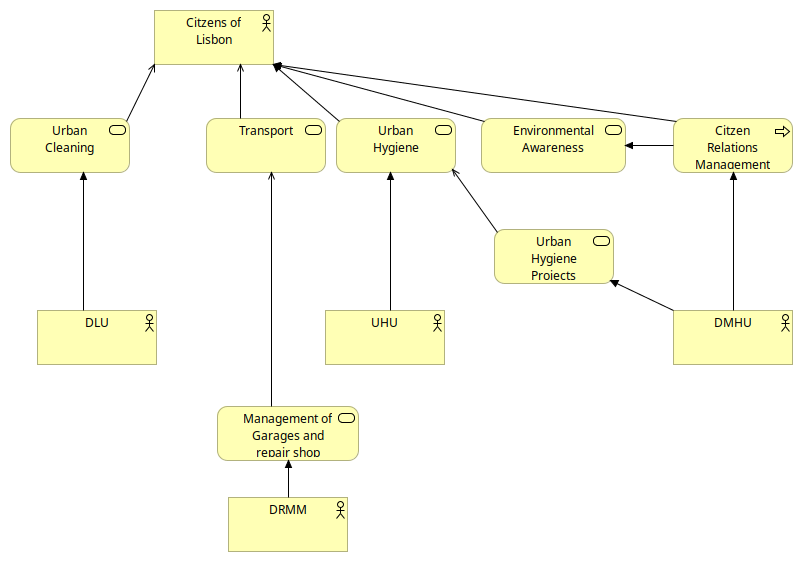
\includegraphics[width=0.6\textwidth]{Q2 - Business Services}
        \caption{Serviços Prestados pela DMHU}
        \label{fig:2}
    \end{figure}

    Estes serviços respondem às necessidades operacionais do município e estão alinhados com os objetivos estratégicos definidos no Relatório de Atividades de 2015.
    Esta descrição responde à \textbf{Questão 2 — Product Viewpoint}.

    \newpage

    \section{Estrutura Organizacional da DMHU}\label{sec:estrutura-organizacional-da-dmhu}

    A estrutura da DMHU está dividida em dois departamentos principais:
    \begin{itemize}
        \item \textbf{DHU} – Departamento de Higiene Urbana (inclui DLU e UHU);
        \item \textbf{DRMM} – Departamento de Reparação e Manutenção Mecânica (inclui DGF e DMF).
    \end{itemize}

    \begin{figure}[h!]
        \centering
        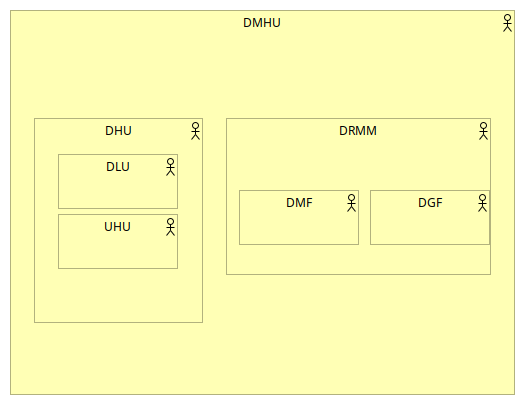
\includegraphics[width=0.85\textwidth]{Q3 - Organizational Structure}
        \caption{Organograma DMHU — Modelo ArchiMate}
        \label{fig:3}
    \end{figure}

    Esta estrutura foi validada com base na documentação oficial de 2019 e responde à \textbf{Questão 3 — Organization Viewpoint}.

    \newpage
    \section{Processos e Relação com os Serviços}\label{sec:processos-e-relacao-com-os-servicos}

    Os serviços identificados anteriormente são suportados por cinco macroprocessos:
    \begin{itemize}
        \item Gestão da Recolha de Resíduos;
        \item Relação com o Cidadão;
        \item Gestão de Recursos Humanos;
        \item Gestão do Armazém;
        \item Gestão da Frota.
    \end{itemize}

    \begin{figure}[ht!]
        \centering
        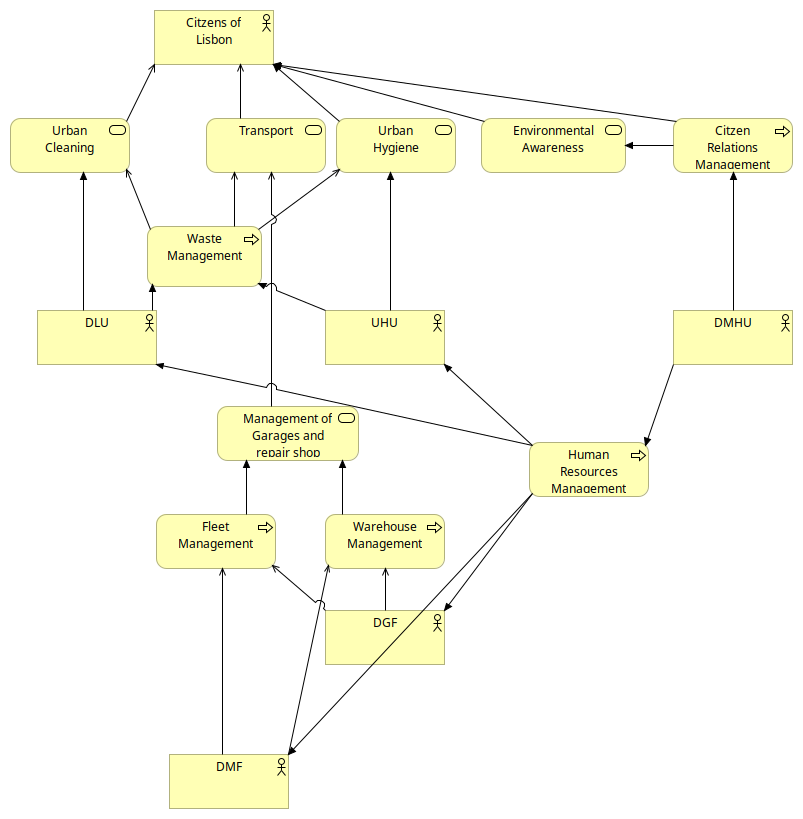
\includegraphics[width=0.65\textwidth]{Q4 - Relation Between Business services and Business Processes}
        \caption{Relação entre Serviços e Processos}
        \label{fig:4}
    \end{figure}
    Esta associação entre serviços e processos responde à \textbf{Questão 4 — Service-Process Viewpoint}.

    \newpage
    \section{Especificação dos Processos de Negócio}\label{sec:especificacao-dos-processos-de-negocio}

    Cada macroprocesso inclui subprocessos detalhados:
    \begin{itemize}
        \item Recolha de Resíduos: Planeamento, Execução, Registo;
        \item Relação com o Cidadão: Interação com GOPI, Avaliação de Pedidos;
        \item Recursos Humanos: Registos, Formação, Férias, Fardamento;
        \item Frota: Manutenção, Alocação de Viaturas;
        \item Armazém: Gestão de Stocks, Requisições, Armazenamento.
    \end{itemize}

    \begin{figure}[ht!]
        \centering
        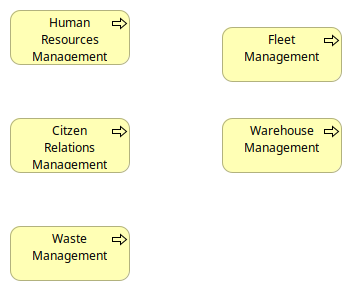
\includegraphics[width=0.6\textwidth]{Q5 - High Level Specification of Business Process}
        \caption{Modelo de Processos de Negócio — ArchiMate}
        \label{fig:5}
    \end{figure}

    Este modelo detalha os fluxos de trabalho internos e responde à \textbf{Questão 5 — Business Process Viewpoint}.


\end{document}